\section{Objects in the amber.crawler package}

\classname{Configuration}

\begin{classmetadata}
\end{classmetadata}

\begin{interface}
\end{interface}



\classname{RSS}

\begin{classmetadata}
  \extends{amber.CrawlerObject}
  \implements{amber.common.AirBrushCallable}
\end{classmetadata}

\begin{interface}
  \method{Boolean}{addFeed}{URL}
    {Adds a feed to the crawler. Will be crawled during the next cycle. Returns
      true if succesful, false otherwise.}
  \method{Boolean}{removeFeed}{}{FIXME: do or don't?}
\end{interface}



\begin{figure}
  \centering
  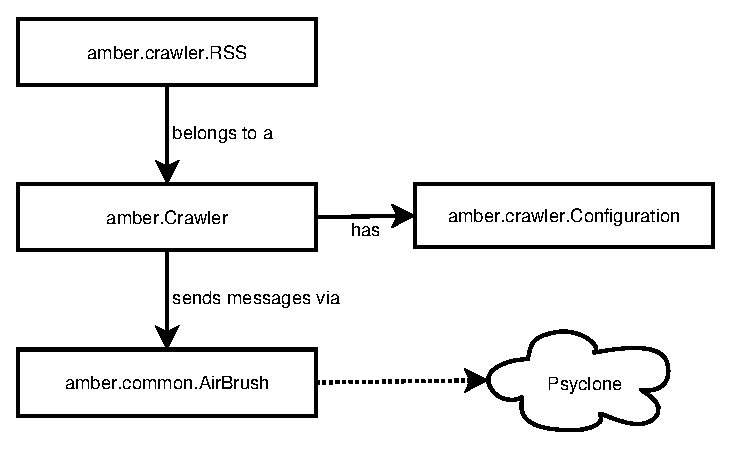
\includegraphics{image/crawler}
  \caption{
    Diagram of the design of the Crawler, the names are Java classnames
  }
\end{figure}

